\documentclass[]{article}
\usepackage{lmodern}
\usepackage{amssymb,amsmath}
\usepackage{ifxetex,ifluatex}
\usepackage{fixltx2e} % provides \textsubscript
\ifnum 0\ifxetex 1\fi\ifluatex 1\fi=0 % if pdftex
  \usepackage[T1]{fontenc}
  \usepackage[utf8]{inputenc}
\else % if luatex or xelatex
  \ifxetex
    \usepackage{mathspec}
  \else
    \usepackage{fontspec}
  \fi
  \defaultfontfeatures{Ligatures=TeX,Scale=MatchLowercase}
\fi
% use upquote if available, for straight quotes in verbatim environments
\IfFileExists{upquote.sty}{\usepackage{upquote}}{}
% use microtype if available
\IfFileExists{microtype.sty}{%
\usepackage{microtype}
\UseMicrotypeSet[protrusion]{basicmath} % disable protrusion for tt fonts
}{}
\usepackage[margin=1in]{geometry}
\usepackage{hyperref}
\hypersetup{unicode=true,
            pdftitle={Computing sparse eigenvectors},
            pdfauthor={Konstantinos Benidis and Daniel P. Palomar},
            pdfborder={0 0 0},
            breaklinks=true}
\urlstyle{same}  % don't use monospace font for urls
\usepackage{color}
\usepackage{fancyvrb}
\newcommand{\VerbBar}{|}
\newcommand{\VERB}{\Verb[commandchars=\\\{\}]}
\DefineVerbatimEnvironment{Highlighting}{Verbatim}{commandchars=\\\{\}}
% Add ',fontsize=\small' for more characters per line
\usepackage{framed}
\definecolor{shadecolor}{RGB}{248,248,248}
\newenvironment{Shaded}{\begin{snugshade}}{\end{snugshade}}
\newcommand{\KeywordTok}[1]{\textcolor[rgb]{0.13,0.29,0.53}{\textbf{#1}}}
\newcommand{\DataTypeTok}[1]{\textcolor[rgb]{0.13,0.29,0.53}{#1}}
\newcommand{\DecValTok}[1]{\textcolor[rgb]{0.00,0.00,0.81}{#1}}
\newcommand{\BaseNTok}[1]{\textcolor[rgb]{0.00,0.00,0.81}{#1}}
\newcommand{\FloatTok}[1]{\textcolor[rgb]{0.00,0.00,0.81}{#1}}
\newcommand{\ConstantTok}[1]{\textcolor[rgb]{0.00,0.00,0.00}{#1}}
\newcommand{\CharTok}[1]{\textcolor[rgb]{0.31,0.60,0.02}{#1}}
\newcommand{\SpecialCharTok}[1]{\textcolor[rgb]{0.00,0.00,0.00}{#1}}
\newcommand{\StringTok}[1]{\textcolor[rgb]{0.31,0.60,0.02}{#1}}
\newcommand{\VerbatimStringTok}[1]{\textcolor[rgb]{0.31,0.60,0.02}{#1}}
\newcommand{\SpecialStringTok}[1]{\textcolor[rgb]{0.31,0.60,0.02}{#1}}
\newcommand{\ImportTok}[1]{#1}
\newcommand{\CommentTok}[1]{\textcolor[rgb]{0.56,0.35,0.01}{\textit{#1}}}
\newcommand{\DocumentationTok}[1]{\textcolor[rgb]{0.56,0.35,0.01}{\textbf{\textit{#1}}}}
\newcommand{\AnnotationTok}[1]{\textcolor[rgb]{0.56,0.35,0.01}{\textbf{\textit{#1}}}}
\newcommand{\CommentVarTok}[1]{\textcolor[rgb]{0.56,0.35,0.01}{\textbf{\textit{#1}}}}
\newcommand{\OtherTok}[1]{\textcolor[rgb]{0.56,0.35,0.01}{#1}}
\newcommand{\FunctionTok}[1]{\textcolor[rgb]{0.00,0.00,0.00}{#1}}
\newcommand{\VariableTok}[1]{\textcolor[rgb]{0.00,0.00,0.00}{#1}}
\newcommand{\ControlFlowTok}[1]{\textcolor[rgb]{0.13,0.29,0.53}{\textbf{#1}}}
\newcommand{\OperatorTok}[1]{\textcolor[rgb]{0.81,0.36,0.00}{\textbf{#1}}}
\newcommand{\BuiltInTok}[1]{#1}
\newcommand{\ExtensionTok}[1]{#1}
\newcommand{\PreprocessorTok}[1]{\textcolor[rgb]{0.56,0.35,0.01}{\textit{#1}}}
\newcommand{\AttributeTok}[1]{\textcolor[rgb]{0.77,0.63,0.00}{#1}}
\newcommand{\RegionMarkerTok}[1]{#1}
\newcommand{\InformationTok}[1]{\textcolor[rgb]{0.56,0.35,0.01}{\textbf{\textit{#1}}}}
\newcommand{\WarningTok}[1]{\textcolor[rgb]{0.56,0.35,0.01}{\textbf{\textit{#1}}}}
\newcommand{\AlertTok}[1]{\textcolor[rgb]{0.94,0.16,0.16}{#1}}
\newcommand{\ErrorTok}[1]{\textcolor[rgb]{0.64,0.00,0.00}{\textbf{#1}}}
\newcommand{\NormalTok}[1]{#1}
\usepackage{graphicx,grffile}
\makeatletter
\def\maxwidth{\ifdim\Gin@nat@width>\linewidth\linewidth\else\Gin@nat@width\fi}
\def\maxheight{\ifdim\Gin@nat@height>\textheight\textheight\else\Gin@nat@height\fi}
\makeatother
% Scale images if necessary, so that they will not overflow the page
% margins by default, and it is still possible to overwrite the defaults
% using explicit options in \includegraphics[width, height, ...]{}
\setkeys{Gin}{width=\maxwidth,height=\maxheight,keepaspectratio}
\IfFileExists{parskip.sty}{%
\usepackage{parskip}
}{% else
\setlength{\parindent}{0pt}
\setlength{\parskip}{6pt plus 2pt minus 1pt}
}
\setlength{\emergencystretch}{3em}  % prevent overfull lines
\providecommand{\tightlist}{%
  \setlength{\itemsep}{0pt}\setlength{\parskip}{0pt}}
\setcounter{secnumdepth}{5}
% Redefines (sub)paragraphs to behave more like sections
\ifx\paragraph\undefined\else
\let\oldparagraph\paragraph
\renewcommand{\paragraph}[1]{\oldparagraph{#1}\mbox{}}
\fi
\ifx\subparagraph\undefined\else
\let\oldsubparagraph\subparagraph
\renewcommand{\subparagraph}[1]{\oldsubparagraph{#1}\mbox{}}
\fi

%%% Use protect on footnotes to avoid problems with footnotes in titles
\let\rmarkdownfootnote\footnote%
\def\footnote{\protect\rmarkdownfootnote}

%%% Change title format to be more compact
\usepackage{titling}

% Create subtitle command for use in maketitle
\newcommand{\subtitle}[1]{
  \posttitle{
    \begin{center}\large#1\end{center}
    }
}

\setlength{\droptitle}{-2em}
  \title{Computing sparse eigenvectors}
  \pretitle{\vspace{\droptitle}\centering\huge}
  \posttitle{\par}
  \author{Konstantinos Benidis and Daniel P. Palomar}
  \preauthor{\centering\large\emph}
  \postauthor{\par}
  \predate{\centering\large\emph}
  \postdate{\par}
  \date{2017-12-07}

\setlength{\parindent}{12pt} \usepackage{graphicx}

\begin{document}
\maketitle

{
\setcounter{tocdepth}{2}
\tableofcontents
}
\begin{center}\rule{0.5\linewidth}{\linethickness}\end{center}

This vignette illustrates the computation of sparse eigenvectors or
sparse PCA with the package \texttt{sparseEigen} (with a comparison with
other packages) and gives a description of the algorithms used.

\section{Comparison with other
packages}\label{comparison-with-other-packages}

We compare the proposed function \texttt{spEigen()} with the functions
\texttt{elasticnet::spca()} and \texttt{rrcovHD::SPcaGrid()}.

First, we illustrate how the functions scale with dimension. For this,
we generate synthetic data with sparse eigenvectors (see next section
for details) of increasing dimension (100 Monte Carlo runs in each
dimension). We apply the two functions to extract the first three
eigenvectors. The figure below illustrates how the running time of the
functions increase as we increase the dimension of the problem. It is
clear that \texttt{spEigen()} scales very well, while
\texttt{SPcaGrid()} and \texttt{spca()} become impractical for large
dimensions.

\begin{center}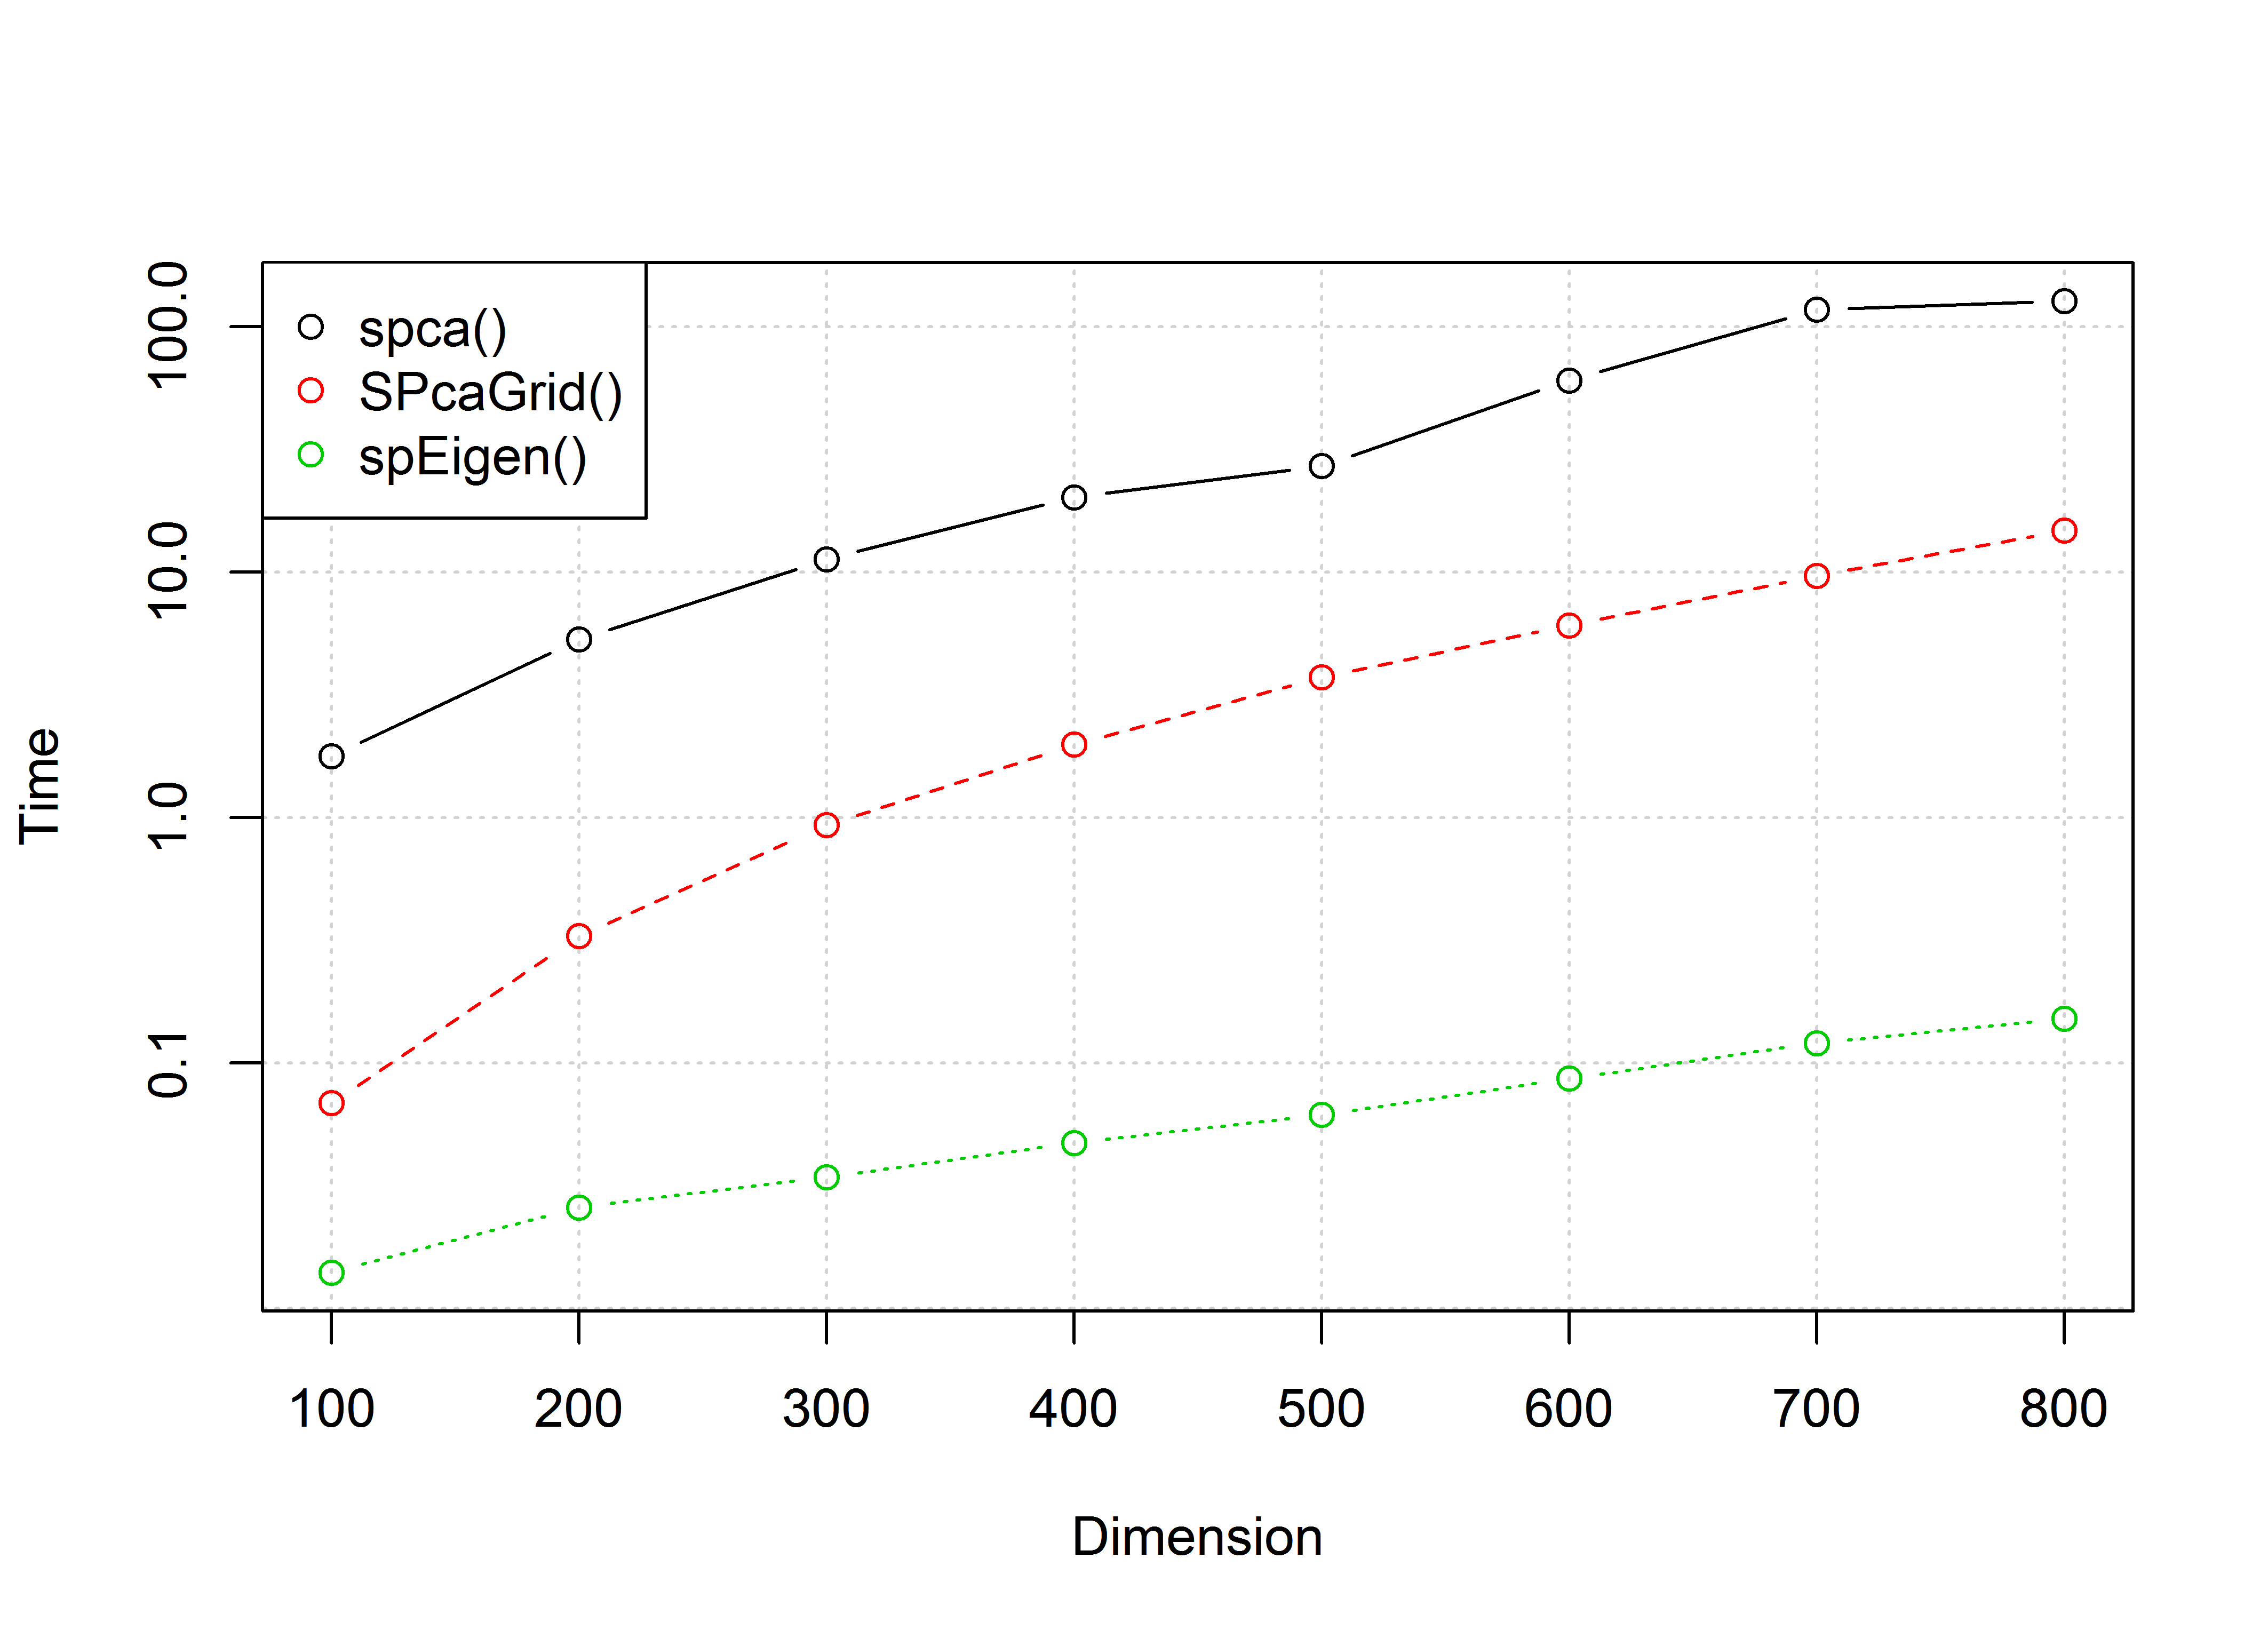
\includegraphics[width=0.75\linewidth]{figures/running_time} \end{center}

Another advantage of \texttt{spEigen()} (and \texttt{spEigenCov()}) is
the parsimony and robustness in parameter selection. To illustrate this,
in the next figure we compare the angle and pattern recovery ability of
the functions. To this end, we generate 200 samples form a multivariate
Gaussian distribution of dimension 500, following the process described
in the next section.

\begin{center}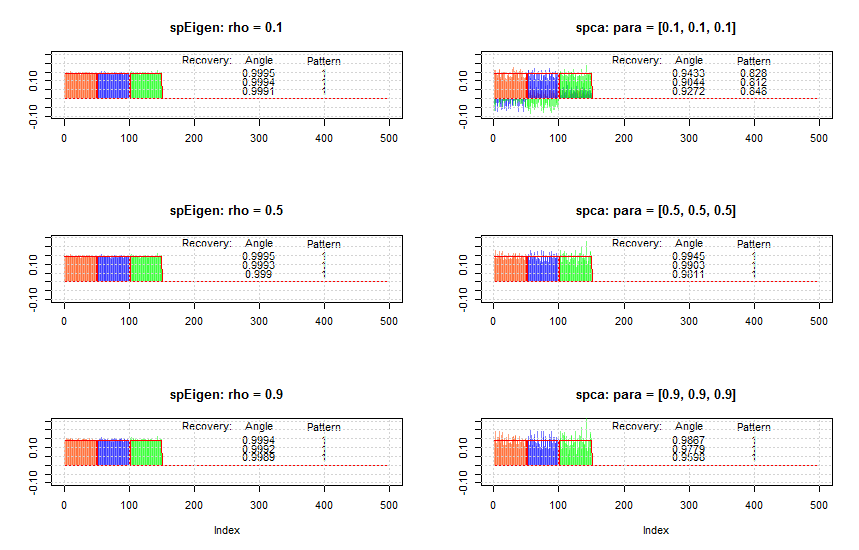
\includegraphics[width=0.95\linewidth]{figures/recovery} \end{center}

We observe that \texttt{spEigen()} requires only one parameter and can
recover correctly the eigenvectors for a large range of the parameter's
values. On the other hand, \texttt{spca()} requires one parameter per
eigenvector, the recovery is significantly affected by small changes of
these parameters, and in general it underperforms compared to
\texttt{spEigen()}. Finally, \texttt{SPcaGrid()} requires one sparsity
parameter (it also accepts one parameter per eigenvector) but cannot
capture efficiently the sparsity pattern of the eigenvectors.

Further advantages of \texttt{spEigen()} are that it can handle real and
complex data, and it accepts as input both data and covariance matrices.

\section{Usage of the package}\label{usage-of-the-package}

\subsection{Computation of sparse eigenvectors of a given
matrix}\label{computation-of-sparse-eigenvectors-of-a-given-matrix}

We start by loading the package and generating synthetic data with
sparse eigenvectors:

\begin{Shaded}
\begin{Highlighting}[]
\KeywordTok{library}\NormalTok{(sparseEigen)}
\KeywordTok{set.seed}\NormalTok{(}\DecValTok{42}\NormalTok{)}

\CommentTok{# parameters }
\NormalTok{m <-}\StringTok{ }\DecValTok{500}  \CommentTok{# dimension}
\NormalTok{n <-}\StringTok{ }\DecValTok{100}  \CommentTok{# number of samples}
\NormalTok{q <-}\StringTok{ }\DecValTok{3}  \CommentTok{# number of sparse eigenvectors to be estimated}
\NormalTok{sp_card <-}\StringTok{ }\FloatTok{0.2}\OperatorTok{*}\NormalTok{m  }\CommentTok{# cardinality of each sparse eigenvector}
\NormalTok{rho <-}\StringTok{ }\FloatTok{0.6}  \CommentTok{# sparsity level}

\CommentTok{# generate non-overlapping sparse eigenvectors}
\NormalTok{V <-}\StringTok{ }\KeywordTok{matrix}\NormalTok{(}\DecValTok{0}\NormalTok{, m, q)}
\NormalTok{V[}\KeywordTok{cbind}\NormalTok{(}\KeywordTok{seq}\NormalTok{(}\DecValTok{1}\NormalTok{, q}\OperatorTok{*}\NormalTok{sp_card), }\KeywordTok{rep}\NormalTok{(}\DecValTok{1}\OperatorTok{:}\NormalTok{q, }\DataTypeTok{each =}\NormalTok{ sp_card))] <-}\StringTok{ }\DecValTok{1}\OperatorTok{/}\KeywordTok{sqrt}\NormalTok{(sp_card)}
\NormalTok{V <-}\StringTok{ }\KeywordTok{cbind}\NormalTok{(V, }\KeywordTok{matrix}\NormalTok{(}\KeywordTok{rnorm}\NormalTok{(m}\OperatorTok{*}\NormalTok{(m}\OperatorTok{-}\NormalTok{q)), m, m}\OperatorTok{-}\NormalTok{q))}
\CommentTok{# keep first q eigenvectors the same (already orthogonal) and orthogonalize the rest}
\NormalTok{V <-}\StringTok{ }\KeywordTok{qr.Q}\NormalTok{(}\KeywordTok{qr}\NormalTok{(V))}

\CommentTok{# generate eigenvalues}
\NormalTok{lmd <-}\StringTok{ }\KeywordTok{c}\NormalTok{(}\DecValTok{100}\OperatorTok{*}\KeywordTok{seq}\NormalTok{(}\DataTypeTok{from =}\NormalTok{ q, }\DataTypeTok{to =} \DecValTok{1}\NormalTok{), }\KeywordTok{rep}\NormalTok{(}\DecValTok{1}\NormalTok{, m}\OperatorTok{-}\NormalTok{q))}

\CommentTok{# generate covariance matrix from sparse eigenvectors and eigenvalues}
\NormalTok{R <-}\StringTok{ }\NormalTok{V }\OperatorTok\StringTok{ }\KeywordTok{diag}\NormalTok{(lmd) }\OperatorTok\StringTok{ }\KeywordTok{t}\NormalTok{(V)}

\CommentTok{# generate data matrix from a zero-mean multivariate Gaussian distribution }
\CommentTok{# with the constructed covariance}
\NormalTok{X <-}\StringTok{ }\NormalTok{MASS}\OperatorTok{::}\KeywordTok{mvrnorm}\NormalTok{(n, }\KeywordTok{rep}\NormalTok{(}\DecValTok{0}\NormalTok{, m), R)  }\CommentTok{# random data with underlying sparse structure}
\end{Highlighting}
\end{Shaded}

Then, we estimate the covariance matrix with \texttt{cov(X)} and compute
its sparse eigenvectors with \texttt{spEigen()}:

\begin{Shaded}
\begin{Highlighting}[]
\CommentTok{# computation of sparse eigenvectors}
\NormalTok{res_standard <-}\StringTok{ }\KeywordTok{eigen}\NormalTok{(}\KeywordTok{cov}\NormalTok{(X))}
\NormalTok{res_sparse1 <-}\StringTok{ }\KeywordTok{spEigen}\NormalTok{(}\KeywordTok{cov}\NormalTok{(X), q, rho)}
\NormalTok{res_sparse2 <-}\StringTok{ }\KeywordTok{spEigen}\NormalTok{(X, q, rho, }\DataTypeTok{data =} \OtherTok{TRUE}\NormalTok{)}
\end{Highlighting}
\end{Shaded}

We can assess how good the estimated eigenvectors are by computing the
inner product with the original eigenvectors (the closer to 1 the
better):

\begin{Shaded}
\begin{Highlighting}[]
\CommentTok{# show inner product between estimated eigenvectors and originals}
\KeywordTok{abs}\NormalTok{(}\KeywordTok{diag}\NormalTok{(}\KeywordTok{t}\NormalTok{(res_standard}\OperatorTok{$}\NormalTok{vectors) }\OperatorTok\StringTok{ }\NormalTok{V[, }\DecValTok{1}\OperatorTok{:}\NormalTok{q]))   }\CommentTok{#for standard estimated eigenvectors}
\CommentTok{#> [1] 0.9215392 0.9194898 0.9740871}
\KeywordTok{abs}\NormalTok{(}\KeywordTok{diag}\NormalTok{(}\KeywordTok{t}\NormalTok{(res_sparse1}\OperatorTok{$}\NormalTok{vectors) }\OperatorTok\StringTok{ }\NormalTok{V[, }\DecValTok{1}\OperatorTok{:}\NormalTok{q]))    }\CommentTok{#for sparse estimated eigenvectors}
\CommentTok{#> [1] 0.9971771 0.9969985 0.9924857}
\KeywordTok{abs}\NormalTok{(}\KeywordTok{diag}\NormalTok{(}\KeywordTok{t}\NormalTok{(res_sparse2}\OperatorTok{$}\NormalTok{vectors) }\OperatorTok\StringTok{ }\NormalTok{V[, }\DecValTok{1}\OperatorTok{:}\NormalTok{q]))    }\CommentTok{#for sparse estimated eigenvectors}
\CommentTok{#> [1] 0.9971593 0.9969798 0.9924368}
\end{Highlighting}
\end{Shaded}

Finally, the following plot shows the sparsity pattern of the
eigenvectors (sparse computation vs.~classical computation):

\begin{Shaded}
\begin{Highlighting}[]
\KeywordTok{par}\NormalTok{(}\DataTypeTok{mfcol =} \KeywordTok{c}\NormalTok{(}\DecValTok{3}\NormalTok{, }\DecValTok{2}\NormalTok{))}
\KeywordTok{plot}\NormalTok{(res_sparse1}\OperatorTok{$}\NormalTok{vectors[, }\DecValTok{1}\NormalTok{]}\OperatorTok{*}\KeywordTok{sign}\NormalTok{(res_sparse1}\OperatorTok{$}\NormalTok{vectors[}\DecValTok{1}\NormalTok{, }\DecValTok{1}\NormalTok{]), }
     \DataTypeTok{main =} \StringTok{"First sparse eigenvector"}\NormalTok{, }\DataTypeTok{xlab =} \StringTok{"index"}\NormalTok{, }\DataTypeTok{ylab =} \StringTok{""}\NormalTok{, }\DataTypeTok{type =} \StringTok{"h"}\NormalTok{)}
\KeywordTok{lines}\NormalTok{(V[, }\DecValTok{1}\NormalTok{]}\OperatorTok{*}\KeywordTok{sign}\NormalTok{(V[}\DecValTok{1}\NormalTok{, }\DecValTok{1}\NormalTok{]), }\DataTypeTok{col =} \StringTok{"red"}\NormalTok{)}
\KeywordTok{plot}\NormalTok{(res_sparse1}\OperatorTok{$}\NormalTok{vectors[, }\DecValTok{2}\NormalTok{]}\OperatorTok{*}\KeywordTok{sign}\NormalTok{(res_sparse1}\OperatorTok{$}\NormalTok{vectors[sp_card}\OperatorTok{+}\DecValTok{1}\NormalTok{, }\DecValTok{2}\NormalTok{]), }
     \DataTypeTok{main =} \StringTok{"Second sparse eigenvector"}\NormalTok{, }\DataTypeTok{xlab =} \StringTok{"index"}\NormalTok{, }\DataTypeTok{ylab =} \StringTok{""}\NormalTok{, }\DataTypeTok{type =} \StringTok{"h"}\NormalTok{)}
\KeywordTok{lines}\NormalTok{(V[, }\DecValTok{2}\NormalTok{]}\OperatorTok{*}\KeywordTok{sign}\NormalTok{(V[sp_card}\OperatorTok{+}\DecValTok{1}\NormalTok{, }\DecValTok{2}\NormalTok{]), }\DataTypeTok{col =} \StringTok{"red"}\NormalTok{)}
\KeywordTok{plot}\NormalTok{(res_sparse1}\OperatorTok{$}\NormalTok{vectors[, }\DecValTok{3}\NormalTok{]}\OperatorTok{*}\KeywordTok{sign}\NormalTok{(res_sparse1}\OperatorTok{$}\NormalTok{vectors[}\DecValTok{2}\OperatorTok{*}\NormalTok{sp_card}\OperatorTok{+}\DecValTok{1}\NormalTok{, }\DecValTok{3}\NormalTok{]), }
     \DataTypeTok{main =} \StringTok{"Third sparse eigenvector"}\NormalTok{, }\DataTypeTok{xlab =} \StringTok{"index"}\NormalTok{, }\DataTypeTok{ylab =} \StringTok{""}\NormalTok{, }\DataTypeTok{type =} \StringTok{"h"}\NormalTok{)}
\KeywordTok{lines}\NormalTok{(V[, }\DecValTok{3}\NormalTok{]}\OperatorTok{*}\KeywordTok{sign}\NormalTok{(V[}\DecValTok{2}\OperatorTok{*}\NormalTok{sp_card}\OperatorTok{+}\DecValTok{1}\NormalTok{, }\DecValTok{3}\NormalTok{]), }\DataTypeTok{col =} \StringTok{"red"}\NormalTok{)}

\KeywordTok{plot}\NormalTok{(res_standard}\OperatorTok{$}\NormalTok{vectors[, }\DecValTok{1}\NormalTok{]}\OperatorTok{*}\KeywordTok{sign}\NormalTok{(res_standard}\OperatorTok{$}\NormalTok{vectors[}\DecValTok{1}\NormalTok{, }\DecValTok{1}\NormalTok{]), }
     \DataTypeTok{main =} \StringTok{"First regular eigenvector"}\NormalTok{, }\DataTypeTok{xlab =} \StringTok{"index"}\NormalTok{, }\DataTypeTok{ylab =} \StringTok{""}\NormalTok{, }\DataTypeTok{type =} \StringTok{"h"}\NormalTok{)}
\KeywordTok{lines}\NormalTok{(V[, }\DecValTok{1}\NormalTok{]}\OperatorTok{*}\KeywordTok{sign}\NormalTok{(V[}\DecValTok{1}\NormalTok{, }\DecValTok{1}\NormalTok{]), }\DataTypeTok{col =} \StringTok{"red"}\NormalTok{)}
\KeywordTok{plot}\NormalTok{(res_standard}\OperatorTok{$}\NormalTok{vectors[, }\DecValTok{2}\NormalTok{]}\OperatorTok{*}\KeywordTok{sign}\NormalTok{(res_standard}\OperatorTok{$}\NormalTok{vectors[sp_card}\OperatorTok{+}\DecValTok{1}\NormalTok{, }\DecValTok{2}\NormalTok{]), }
     \DataTypeTok{main =} \StringTok{"Second regular eigenvector"}\NormalTok{, }\DataTypeTok{xlab =} \StringTok{"index"}\NormalTok{, }\DataTypeTok{ylab =} \StringTok{""}\NormalTok{, }\DataTypeTok{type =} \StringTok{"h"}\NormalTok{)}
\KeywordTok{lines}\NormalTok{(V[, }\DecValTok{2}\NormalTok{]}\OperatorTok{*}\KeywordTok{sign}\NormalTok{(V[sp_card}\OperatorTok{+}\DecValTok{1}\NormalTok{, }\DecValTok{2}\NormalTok{]), }\DataTypeTok{col =} \StringTok{"red"}\NormalTok{)}
\KeywordTok{plot}\NormalTok{(res_standard}\OperatorTok{$}\NormalTok{vectors[, }\DecValTok{3}\NormalTok{]}\OperatorTok{*}\KeywordTok{sign}\NormalTok{(res_standard}\OperatorTok{$}\NormalTok{vectors[}\DecValTok{2}\OperatorTok{*}\NormalTok{sp_card}\OperatorTok{+}\DecValTok{1}\NormalTok{, }\DecValTok{3}\NormalTok{]), }
     \DataTypeTok{main =} \StringTok{"Third regular eigenvector"}\NormalTok{, }\DataTypeTok{xlab =} \StringTok{"index"}\NormalTok{, }\DataTypeTok{ylab =} \StringTok{""}\NormalTok{, }\DataTypeTok{type =} \StringTok{"h"}\NormalTok{)}
\KeywordTok{lines}\NormalTok{(V[, }\DecValTok{3}\NormalTok{]}\OperatorTok{*}\KeywordTok{sign}\NormalTok{(V[}\DecValTok{2}\OperatorTok{*}\NormalTok{sp_card}\OperatorTok{+}\DecValTok{1}\NormalTok{, }\DecValTok{3}\NormalTok{]), }\DataTypeTok{col =} \StringTok{"red"}\NormalTok{)}
\end{Highlighting}
\end{Shaded}

\begin{center}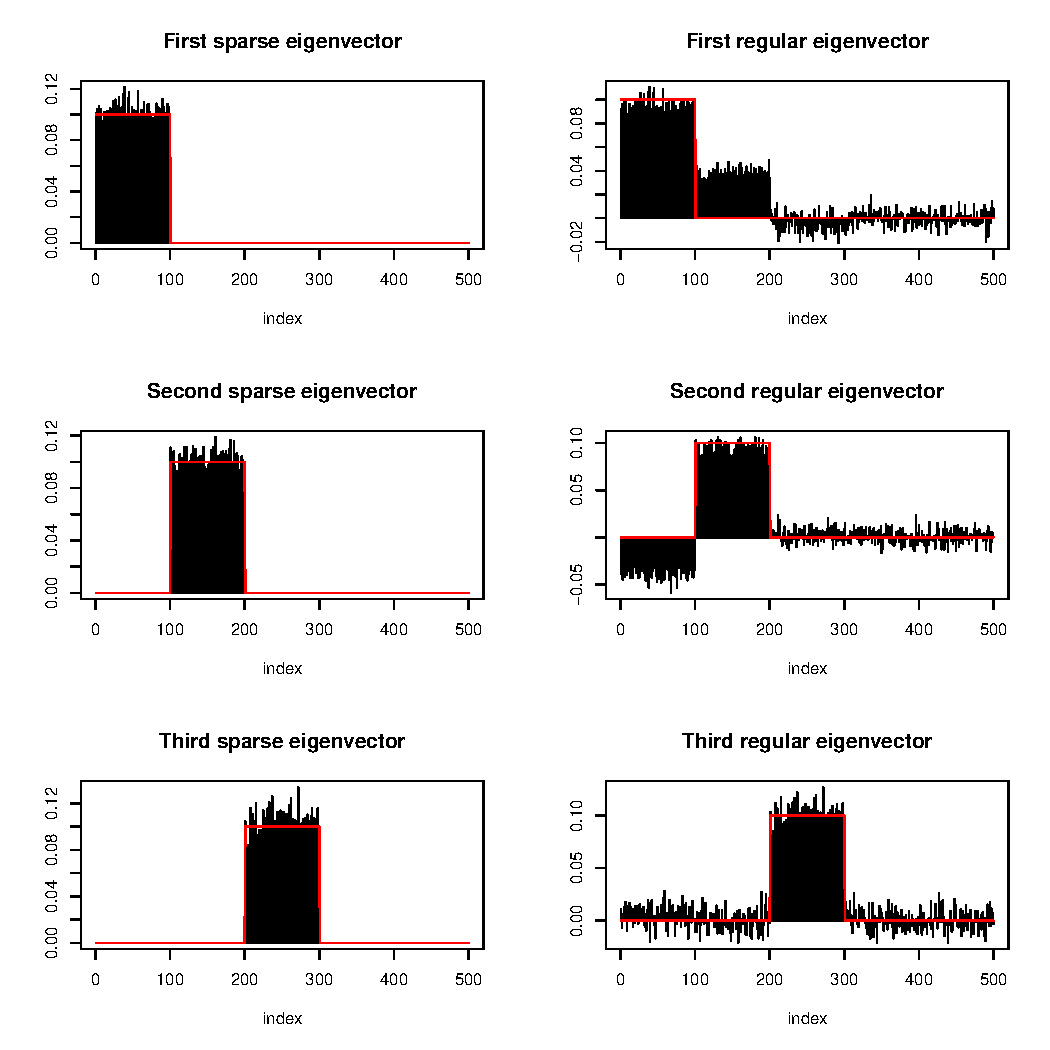
\includegraphics{SparseEigenvectors_files/figure-latex/unnamed-chunk-7-1} \end{center}

\subsection{Covariance matrix estimation with sparse
eigenvectors}\label{covariance-matrix-estimation-with-sparse-eigenvectors}

The function \texttt{spEigenCov()} requires more samples than the
dimension (otherwise some regularization is required). Therefore, we
generate data as previously with the only difference that we set the
number of samples to be \texttt{n=600}.

Then, we compute the covariance matrix through the joint estimation of
sparse eigenvectors and eigenvalues:

\begin{Shaded}
\begin{Highlighting}[]
\CommentTok{# computation of covariance matrix}
\NormalTok{res_sparse3 <-}\StringTok{ }\KeywordTok{spEigenCov}\NormalTok{(}\KeywordTok{cov}\NormalTok{(X), q, rho)}
\end{Highlighting}
\end{Shaded}

Again, we can assess how good the estimated eigenvectors are by
computing the inner product with the original eigenvectors:

\begin{Shaded}
\begin{Highlighting}[]
\CommentTok{# show inner product between estimated eigenvectors and originals}
\KeywordTok{abs}\NormalTok{(}\KeywordTok{diag}\NormalTok{(}\KeywordTok{t}\NormalTok{(res_sparse3}\OperatorTok{$}\NormalTok{vectors[, }\DecValTok{1}\OperatorTok{:}\NormalTok{q]) }\OperatorTok\StringTok{ }\NormalTok{V[, }\DecValTok{1}\OperatorTok{:}\NormalTok{q]))    }\CommentTok{#for sparse estimated eigenvectors}
\CommentTok{#> [1] 0.9994578 0.9990208 0.9985083}
\end{Highlighting}
\end{Shaded}

The following plot shows the sparsity pattern of the eigenvectors:

\begin{Shaded}
\begin{Highlighting}[]
\KeywordTok{par}\NormalTok{(}\DataTypeTok{mfcol =} \KeywordTok{c}\NormalTok{(}\DecValTok{3}\NormalTok{, }\DecValTok{1}\NormalTok{))}
\KeywordTok{plot}\NormalTok{(res_sparse3}\OperatorTok{$}\NormalTok{vectors[, }\DecValTok{1}\NormalTok{]}\OperatorTok{*}\KeywordTok{sign}\NormalTok{(res_sparse3}\OperatorTok{$}\NormalTok{vectors[}\DecValTok{1}\NormalTok{, }\DecValTok{1}\NormalTok{]), }
     \DataTypeTok{main =} \StringTok{"First sparse eigenvector"}\NormalTok{, }\DataTypeTok{xlab =} \StringTok{"index"}\NormalTok{, }\DataTypeTok{ylab =} \StringTok{""}\NormalTok{, }\DataTypeTok{type =} \StringTok{"h"}\NormalTok{)}
\KeywordTok{lines}\NormalTok{(V[, }\DecValTok{1}\NormalTok{]}\OperatorTok{*}\KeywordTok{sign}\NormalTok{(V[}\DecValTok{1}\NormalTok{, }\DecValTok{1}\NormalTok{]), }\DataTypeTok{col =} \StringTok{"red"}\NormalTok{)}
\KeywordTok{plot}\NormalTok{(res_sparse3}\OperatorTok{$}\NormalTok{vectors[, }\DecValTok{2}\NormalTok{]}\OperatorTok{*}\KeywordTok{sign}\NormalTok{(res_sparse3}\OperatorTok{$}\NormalTok{vectors[sp_card}\OperatorTok{+}\DecValTok{1}\NormalTok{, }\DecValTok{2}\NormalTok{]), }
     \DataTypeTok{main =} \StringTok{"Second sparse eigenvector"}\NormalTok{, }\DataTypeTok{xlab =} \StringTok{"index"}\NormalTok{, }\DataTypeTok{ylab =} \StringTok{""}\NormalTok{, }\DataTypeTok{type =} \StringTok{"h"}\NormalTok{)}
\KeywordTok{lines}\NormalTok{(V[, }\DecValTok{2}\NormalTok{]}\OperatorTok{*}\KeywordTok{sign}\NormalTok{(V[sp_card}\OperatorTok{+}\DecValTok{1}\NormalTok{, }\DecValTok{2}\NormalTok{]), }\DataTypeTok{col =} \StringTok{"red"}\NormalTok{)}
\KeywordTok{plot}\NormalTok{(res_sparse3}\OperatorTok{$}\NormalTok{vectors[, }\DecValTok{3}\NormalTok{]}\OperatorTok{*}\KeywordTok{sign}\NormalTok{(res_sparse3}\OperatorTok{$}\NormalTok{vectors[}\DecValTok{2}\OperatorTok{*}\NormalTok{sp_card}\OperatorTok{+}\DecValTok{1}\NormalTok{, }\DecValTok{3}\NormalTok{]), }
     \DataTypeTok{main =} \StringTok{"Third sparse eigenvector"}\NormalTok{, }\DataTypeTok{xlab =} \StringTok{"index"}\NormalTok{, }\DataTypeTok{ylab =} \StringTok{""}\NormalTok{, }\DataTypeTok{type =} \StringTok{"h"}\NormalTok{)}
\KeywordTok{lines}\NormalTok{(V[, }\DecValTok{3}\NormalTok{]}\OperatorTok{*}\KeywordTok{sign}\NormalTok{(V[}\DecValTok{2}\OperatorTok{*}\NormalTok{sp_card}\OperatorTok{+}\DecValTok{1}\NormalTok{, }\DecValTok{3}\NormalTok{]), }\DataTypeTok{col =} \StringTok{"red"}\NormalTok{)}
\end{Highlighting}
\end{Shaded}

\begin{center}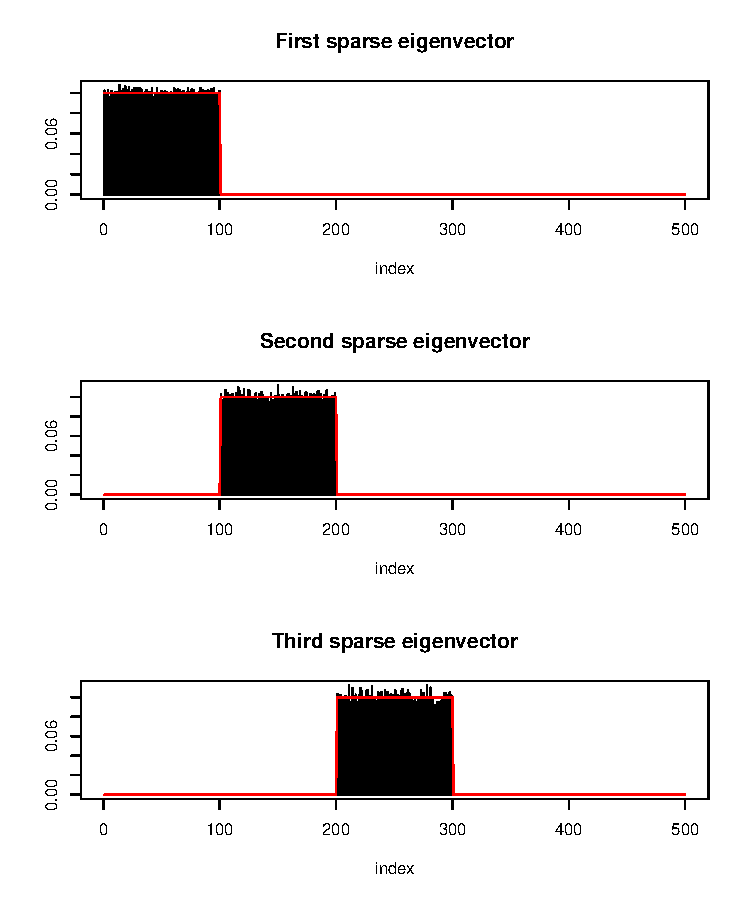
\includegraphics{SparseEigenvectors_files/figure-latex/unnamed-chunk-11-1} \end{center}

Finally, we can compute the error of the estimated covariance matrix
(sparse eigenvector computation vs.~classical computation):

\begin{Shaded}
\begin{Highlighting}[]
\CommentTok{# show error between estimated and true covariance }
\KeywordTok{norm}\NormalTok{(}\KeywordTok{cov}\NormalTok{(X) }\OperatorTok{-}\StringTok{ }\NormalTok{R, }\DataTypeTok{type =} \StringTok{'F'}\NormalTok{) }\CommentTok{#for sample covariance matrix}
\CommentTok{#> [1] 48.42514}
\KeywordTok{norm}\NormalTok{(res_sparse3}\OperatorTok{$}\NormalTok{cov }\OperatorTok{-}\StringTok{ }\NormalTok{R, }\DataTypeTok{type =} \StringTok{'F'}\NormalTok{) }\CommentTok{#for covariance with sparse eigenvectors}
\CommentTok{#> [1] 29.55455}
\end{Highlighting}
\end{Shaded}

\subsection{Complex-valued inputs}\label{complex-valued-inputs}

The previous examples illustrate the usage of the functions
\texttt{spEigen()} and \texttt{spEigenCov()} for real-valued data and
covariance matrices. However, both functions can handle complex-valued
inputs.

Following the previous data generation procedure, we generate sparse
complex eigenvectors by introducing a random phase in each entry:

\begin{Shaded}
\begin{Highlighting}[]
\NormalTok{m <-}\StringTok{ }\DecValTok{500} \CommentTok{# dimension}
\NormalTok{n <-}\StringTok{ }\DecValTok{600} \CommentTok{# number of samples}
\NormalTok{q <-}\StringTok{ }\DecValTok{3} \CommentTok{# number of sparse eigenvectors to be estimated}
\NormalTok{sp_card <-}\StringTok{ }\FloatTok{0.2}\OperatorTok{*}\NormalTok{m }\CommentTok{# cardinality of the sparse eigenvectors}
\NormalTok{rho <-}\StringTok{ }\FloatTok{0.5}

\CommentTok{# generate non-overlapping sparse eigenvectors}
\NormalTok{V <-}\StringTok{ }\KeywordTok{matrix}\NormalTok{(}\DecValTok{0}\NormalTok{, m, q)}
\NormalTok{V[}\KeywordTok{cbind}\NormalTok{(}\KeywordTok{seq}\NormalTok{(}\DecValTok{1}\NormalTok{, q}\OperatorTok{*}\NormalTok{sp_card), }\KeywordTok{rep}\NormalTok{(}\DecValTok{1}\OperatorTok{:}\NormalTok{q, }\DataTypeTok{each =}\NormalTok{ sp_card))] <-}\StringTok{ }
\StringTok{  }\KeywordTok{exp}\NormalTok{(1i}\OperatorTok{*}\KeywordTok{runif}\NormalTok{(q}\OperatorTok{*}\NormalTok{sp_card, }\DecValTok{0}\NormalTok{, }\DecValTok{2}\OperatorTok{*}\NormalTok{pi))}\OperatorTok{/}\KeywordTok{sqrt}\NormalTok{(sp_card)}
\NormalTok{V <-}\StringTok{ }\KeywordTok{cbind}\NormalTok{(V, }\KeywordTok{matrix}\NormalTok{(}\KeywordTok{rnorm}\NormalTok{(m}\OperatorTok{*}\NormalTok{(m}\OperatorTok{-}\NormalTok{q))}\OperatorTok{*}\KeywordTok{exp}\NormalTok{(1i}\OperatorTok{*}\KeywordTok{runif}\NormalTok{(m}\OperatorTok{*}\NormalTok{(m}\OperatorTok{-}\NormalTok{q),}\DecValTok{0}\NormalTok{,}\DecValTok{2}\OperatorTok{*}\NormalTok{pi)), m, m}\OperatorTok{-}\NormalTok{q))}
\CommentTok{# keep first q eigenvectors the same (already orthogonal) and orthogonalize the rest}
\NormalTok{V_ <-}\StringTok{ }\NormalTok{(}\KeywordTok{diag}\NormalTok{(m) }\OperatorTok{-}\StringTok{ }\NormalTok{V[, }\DecValTok{1}\OperatorTok{:}\NormalTok{q] }\OperatorTok\StringTok{ }\KeywordTok{Conj}\NormalTok{(}\KeywordTok{t}\NormalTok{(V[, }\DecValTok{1}\OperatorTok{:}\NormalTok{q]))) }\OperatorTok\StringTok{ }\NormalTok{V[, }\OperatorTok{-}\KeywordTok{c}\NormalTok{(}\DecValTok{1}\OperatorTok{:}\NormalTok{q)]}
\NormalTok{V <-}\StringTok{ }\KeywordTok{cbind}\NormalTok{(V[, }\DecValTok{1}\OperatorTok{:}\NormalTok{q], }\KeywordTok{qr.Q}\NormalTok{(}\KeywordTok{qr}\NormalTok{(V_)))}

\CommentTok{# generate eigenvalues}
\NormalTok{lmd <-}\StringTok{ }\KeywordTok{c}\NormalTok{(}\DecValTok{100}\OperatorTok{*}\KeywordTok{seq}\NormalTok{(}\DataTypeTok{from =}\NormalTok{ q, }\DataTypeTok{to =} \DecValTok{1}\NormalTok{), }\KeywordTok{rep}\NormalTok{(}\DecValTok{1}\NormalTok{, m}\OperatorTok{-}\NormalTok{q))}

\CommentTok{# generate covariance matrix from sparse eigenvectors and eigenvalues}
\NormalTok{R <-}\StringTok{ }\NormalTok{V }\OperatorTok\StringTok{ }\KeywordTok{diag}\NormalTok{(lmd) }\OperatorTok\StringTok{ }\KeywordTok{Conj}\NormalTok{(}\KeywordTok{t}\NormalTok{(V))}

\CommentTok{# generate data matrix from a zero-mean multivariate Gaussian distribution }
\CommentTok{# with the constructed covariance}
\NormalTok{X <-}\StringTok{ }\NormalTok{MASS}\OperatorTok{::}\KeywordTok{mvrnorm}\NormalTok{(n, }\KeywordTok{rep}\NormalTok{(}\DecValTok{0}\NormalTok{, m), R)  }\CommentTok{# random data with underlying sparse structure}
\NormalTok{X <-}\StringTok{ }\KeywordTok{scale}\NormalTok{(X, }\DataTypeTok{center =} \OtherTok{TRUE}\NormalTok{, }\DataTypeTok{scale =} \OtherTok{FALSE}\NormalTok{)}
\end{Highlighting}
\end{Shaded}

Then, we compute the sparse complex eigenvectors (\texttt{spEigen()})
and the covariance matrix (\texttt{spEigenCov()}):

\begin{Shaded}
\begin{Highlighting}[]
\CommentTok{# computation of sparse eigenvectors and covariance matrix}
\NormalTok{S <-}\StringTok{ }\DecValTok{1}\OperatorTok{/}\NormalTok{(n}\OperatorTok{-}\DecValTok{1}\NormalTok{) }\OperatorTok{*}\StringTok{ }\KeywordTok{t}\NormalTok{(X) }\OperatorTok\StringTok{ }\KeywordTok{Conj}\NormalTok{(X)}
\NormalTok{res_sparse4 <-}\StringTok{ }\KeywordTok{spEigen}\NormalTok{(S, q, rho)}
\NormalTok{res_sparse5 <-}\StringTok{ }\KeywordTok{spEigenCov}\NormalTok{(S, q, rho)}
\end{Highlighting}
\end{Shaded}

The following plot shows the sparsity pattern of the eigenvectors for
both functions:

\begin{Shaded}
\begin{Highlighting}[]
\KeywordTok{par}\NormalTok{(}\DataTypeTok{mfcol =} \KeywordTok{c}\NormalTok{(}\DecValTok{3}\NormalTok{, }\DecValTok{2}\NormalTok{))}
\KeywordTok{plot}\NormalTok{(}\KeywordTok{abs}\NormalTok{(res_sparse4}\OperatorTok{$}\NormalTok{vectors[, }\DecValTok{1}\NormalTok{]), }\DataTypeTok{main =} \StringTok{"spEigen: First sparse eigenvector"}\NormalTok{, }
     \DataTypeTok{xlab =} \StringTok{"index"}\NormalTok{, }\DataTypeTok{ylab =} \StringTok{""}\NormalTok{, }\DataTypeTok{type =} \StringTok{"h"}\NormalTok{)}
\KeywordTok{lines}\NormalTok{(}\KeywordTok{abs}\NormalTok{(V[, }\DecValTok{1}\NormalTok{]), }\DataTypeTok{col =} \StringTok{"red"}\NormalTok{)}
\KeywordTok{plot}\NormalTok{(}\KeywordTok{abs}\NormalTok{(res_sparse4}\OperatorTok{$}\NormalTok{vectors[, }\DecValTok{2}\NormalTok{]), }\DataTypeTok{main =} \StringTok{"spEigen: Second sparse eigenvector"}\NormalTok{, }
     \DataTypeTok{xlab =} \StringTok{"index"}\NormalTok{, }\DataTypeTok{ylab =} \StringTok{""}\NormalTok{, }\DataTypeTok{type =} \StringTok{"h"}\NormalTok{)}
\KeywordTok{lines}\NormalTok{(}\KeywordTok{abs}\NormalTok{(V[, }\DecValTok{2}\NormalTok{]), }\DataTypeTok{col =} \StringTok{"red"}\NormalTok{)}
\KeywordTok{plot}\NormalTok{(}\KeywordTok{abs}\NormalTok{(res_sparse4}\OperatorTok{$}\NormalTok{vectors[, }\DecValTok{3}\NormalTok{]), }\DataTypeTok{main =} \StringTok{"spEigen: Third sparse eigenvector"}\NormalTok{, }
     \DataTypeTok{xlab =} \StringTok{"index"}\NormalTok{, }\DataTypeTok{ylab =} \StringTok{""}\NormalTok{, }\DataTypeTok{type =} \StringTok{"h"}\NormalTok{)}
\KeywordTok{lines}\NormalTok{(}\KeywordTok{abs}\NormalTok{(V[, }\DecValTok{3}\NormalTok{]), }\DataTypeTok{col =} \StringTok{"red"}\NormalTok{)}

\KeywordTok{plot}\NormalTok{(}\KeywordTok{abs}\NormalTok{(res_sparse5}\OperatorTok{$}\NormalTok{vectors[, }\DecValTok{1}\NormalTok{]), }\DataTypeTok{main =} \StringTok{"spEigenCov: First sparse eigenvector"}\NormalTok{, }
     \DataTypeTok{xlab =} \StringTok{"index"}\NormalTok{, }\DataTypeTok{ylab =} \StringTok{""}\NormalTok{, }\DataTypeTok{type =} \StringTok{"h"}\NormalTok{)}
\KeywordTok{lines}\NormalTok{(}\KeywordTok{abs}\NormalTok{(V[, }\DecValTok{1}\NormalTok{]), }\DataTypeTok{col =} \StringTok{"red"}\NormalTok{)}
\KeywordTok{plot}\NormalTok{(}\KeywordTok{abs}\NormalTok{(res_sparse5}\OperatorTok{$}\NormalTok{vectors[, }\DecValTok{2}\NormalTok{]), }\DataTypeTok{main =} \StringTok{"spEigenCov: Second sparse eigenvector"}\NormalTok{, }
     \DataTypeTok{xlab =} \StringTok{"index"}\NormalTok{, }\DataTypeTok{ylab =} \StringTok{""}\NormalTok{, }\DataTypeTok{type =} \StringTok{"h"}\NormalTok{)}
\KeywordTok{lines}\NormalTok{(}\KeywordTok{abs}\NormalTok{(V[, }\DecValTok{2}\NormalTok{]), }\DataTypeTok{col =} \StringTok{"red"}\NormalTok{)}
\KeywordTok{plot}\NormalTok{(}\KeywordTok{abs}\NormalTok{(res_sparse5}\OperatorTok{$}\NormalTok{vectors[, }\DecValTok{3}\NormalTok{]), }\DataTypeTok{main =} \StringTok{"spEigenCov: Third sparse eigenvector"}\NormalTok{, }
     \DataTypeTok{xlab =} \StringTok{"index"}\NormalTok{, }\DataTypeTok{ylab =} \StringTok{""}\NormalTok{, }\DataTypeTok{type =} \StringTok{"h"}\NormalTok{)}
\KeywordTok{lines}\NormalTok{(}\KeywordTok{abs}\NormalTok{(V[, }\DecValTok{3}\NormalTok{]), }\DataTypeTok{col =} \StringTok{"red"}\NormalTok{)}
\end{Highlighting}
\end{Shaded}

\begin{center}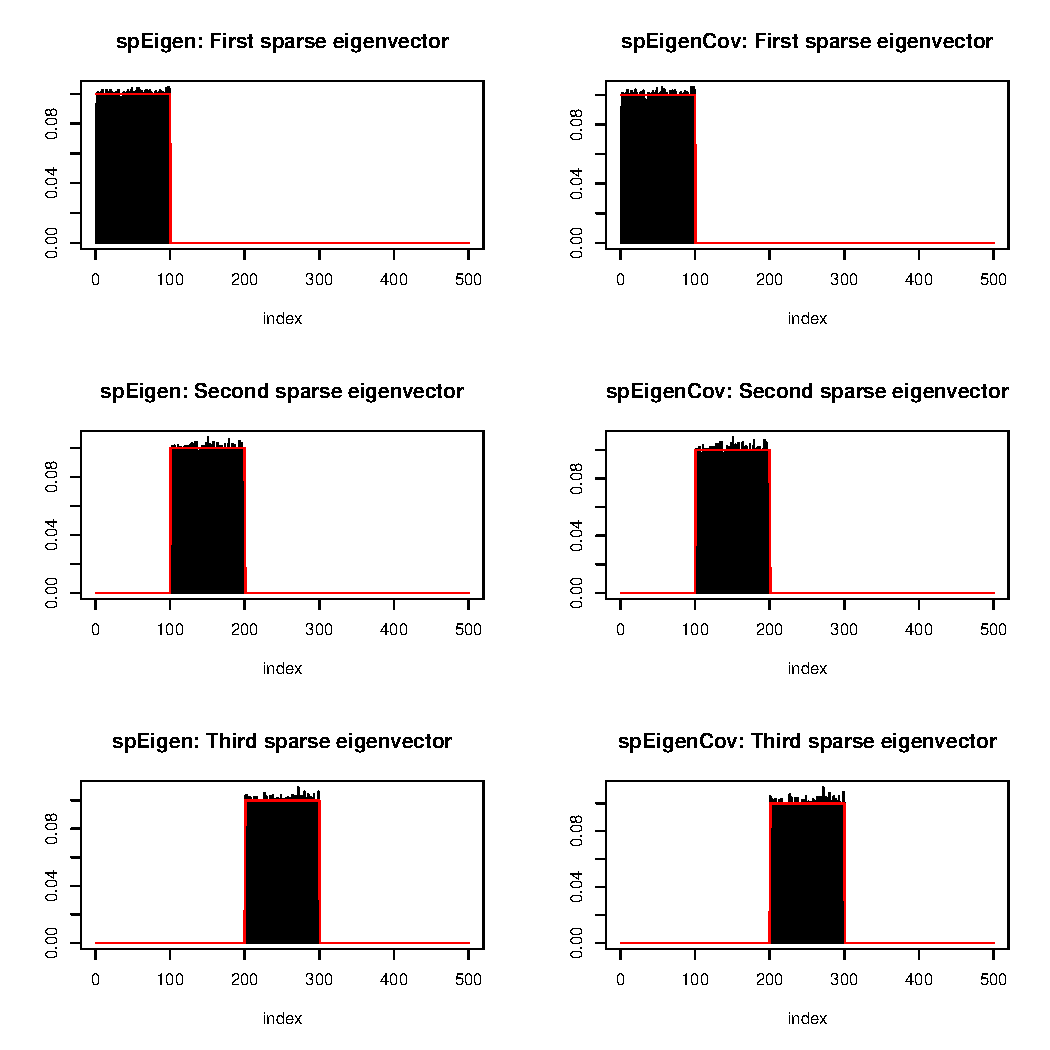
\includegraphics{SparseEigenvectors_files/figure-latex/unnamed-chunk-15-1} \end{center}

Finally, we can compute the error of the estimated covariance matrix
(sparse eigenvector computation vs.~classical computation):

\begin{Shaded}
\begin{Highlighting}[]
\CommentTok{# show error between estimated and true covariance }
\KeywordTok{norm}\NormalTok{(}\KeywordTok{abs}\NormalTok{(S }\OperatorTok{-}\StringTok{ }\NormalTok{R), }\DataTypeTok{type =} \StringTok{'F'}\NormalTok{) }\CommentTok{#for sample covariance matrix}
\CommentTok{#> [1] 50.4656}
\KeywordTok{norm}\NormalTok{(}\KeywordTok{abs}\NormalTok{(res_sparse5}\OperatorTok{$}\NormalTok{cov }\OperatorTok{-}\StringTok{ }\NormalTok{R), }\DataTypeTok{type =} \StringTok{'F'}\NormalTok{) }\CommentTok{#for covariance with sparse eigenvectors}
\CommentTok{#> [1] 28.85653}
\end{Highlighting}
\end{Shaded}

\section{Explanation of the
algorithms}\label{explanation-of-the-algorithms}

\subsection{\texorpdfstring{\texttt{spEigen()}: Sparse eigenvectors from
a given covariance
matrix}{spEigen(): Sparse eigenvectors from a given covariance matrix}}\label{speigen-sparse-eigenvectors-from-a-given-covariance-matrix}

The goal of \texttt{spEigen()} is the estimation of the \(q\) leading
sparse eigenvectors (with \(q \leq \text{rank}(\mathbf{S})\)) from an
\(m\times m\) covariance matrix \(\mathbf{S}\) (typically the sample
covariance matrix obtained from \(n\) samples) based on {[}1{]}. The
underlying optimization problem that is solved is \[\begin{aligned}
      &\underset{\mathbf{U}}{\text{maximize}}\quad \text{Tr} \left(\mathbf{U}^\top \mathbf{S} \mathbf{U} \text{Diag}   (\mathbf{d})\right) - \sum_{i=1}^{q}\rho_i\|\mathbf{u}_i\|_0\\
    &\text{subject to}\quad \mathbf{U}^\top\mathbf{U}=\mathbf{I}_q,
  \end{aligned}\] where \(\mathbf{U}\in\mathbb{R}^{m\times q}\) is a
matrix containing the \(q\) leading eigenvectors, \(\mathbf{d}\) is a
vector of weights to ensure that \(\mathbf{U}\) contains the leading
eigenvectors without an arbitrary rotation, and the \(\rho_i\)'s are the
regularization parameters to control how much sparsity is desired. This
problem is the typical PCA formulation with an extra penalty term in the
objective that penalizes the cardinality of the eigenvectors, controled
by the regularization parameters \(\rho_i\)'s.

The \(\ell_0\)-``norm'' is approximated by the continuous and
differentiable function \[g_p^{\epsilon}\left(x \right)= \begin{cases}
    \frac{x^2}{2\epsilon(p+\epsilon)\log(1+1/p)},& |x|\leq\epsilon,\\
    \frac{\log\left(\frac{p+|x|}{p+\epsilon}\right)+\frac{\epsilon}{2(p+\epsilon)}}{\log(1+1/p)},& |x|>\epsilon,
    \end{cases}\] where \(p>0\) and \(0<\epsilon\ll1\) are parameters
that control the approximation. This leads to the following approximate
problem: \[\begin{aligned}
      &\underset{\mathbf{U}}{\text{maximize}}\quad \text{Tr} \left(\mathbf{U}^\top \mathbf{S} \mathbf{U} \text{Diag}   (\mathbf{d})\right) - \sum_{j=1}^{q}\rho_j\sum_{i=1}^{m}g_p^{\epsilon}\left(u_{ij}\right)\\
    &\text{subject to}\quad \mathbf{U}^\top\mathbf{U}=\mathbf{I}_q.
  \end{aligned}\]

This problem can be solved via Majorization-Minimization (MM) {[}2{]}
with an iterative closed-form update algorithm. For this, at each
iteration (denoted by \(k\)) two key quantities are needed:

\[\mathbf{G}^{(k)} = \mathbf{S}\mathbf{U}^{(k)}\text{Diag}(\mathbf{d})\]\\
\[\mathbf{H}^{(k)}=\left[\text{diag}\left(\mathbf{w}^{(k)}-\mathbf{w}_{\max}^{(k)}\otimes\mathbf{1}_{m}\right)\mathbf{\tilde{u}}^{(k)}\right]_{m\times q},\]
where \[w_{i}^{(k)}= \begin{cases}
        \frac{\rho_i}{2\epsilon(p+\epsilon)\log(1+1/p)},& |\tilde{u}^{(k)}_{i}|\leq\epsilon,\\
        \frac{\rho_i}{2\log(1+1/p)|\tilde{u}^{(k)}_{i}|\left(|\tilde{u}^{(k)}_{i}|+p\right)},&                |\tilde{u}^{(k)}_{i}|>\epsilon,
        \end{cases}\] with \(\mathbf{w}\in\mathbb{R}_+^{mq}\),
\(\mathbf{\tilde{u}}^{(k)} = \text{vec}(\mathbf{U}^{(k)})\in\mathbb{R}_+^{mq}\),
\(\mathbf{w}_{\max}\in\mathbb{R}^q_+\), with \(w_{\max,i}\) being the
maximum weight that corresponds to the \(i\)-th eigenvector
\(\mathbf{u}^{(k)}_{i}\).

The iterative closed-form update algorithm is:

\begin{quote}
\begin{enumerate}
\def\labelenumi{\arabic{enumi}.}
\tightlist
\item
  Set \(k=0\) and choose an initial point \(\mathbf{U}^{(0)}\)\\
\item
  Compute \(\mathbf{G}^{(k)}\) and \(\mathbf{H}^{(k)}\)\\
\item
  Compute \(\mathbf{V}_{\text{L}}\), \(\mathbf{V}_{\text{R}}\) as the
  left and right singular vectors of
  \(\left(\mathbf{G}^{(k)} - \mathbf{H}^{(k)}\right)\)\\
\item
  \(\mathbf{U}^{(k+1)} \gets \mathbf{V}_{\text{L}}\mathbf{V}_{\text{R}}^\top\)\\
\item
  \(k \gets k+1\)\\
\item
  Repeat steps 2-5 until convergence\\
\item
  Return \(\mathbf{U}^{(k)}\)
\end{enumerate}
\end{quote}

The initial point of the algorithm \(\mathbf{U}^{(0)}\) is set by
default to the \(q\) leading standard eigenvectors, unless the user
specifies otherwise. Internally, all the computations of
\(\mathbf{G}^{(k)}\) and \(\mathbf{H}^{(k)}\) are done through the
eigenvalue decomposition (EVD) of \(\mathbf{S}\). Since we can also
retrieve the eigenvectors and eigenvalues of \(\mathbf{S}\) through the
singular value decomposition (SVD) of the data matrix \(\mathbf{X}\),
with \(\mathbf{S} = \frac{1}{n-1}\mathbf{X}^\top\mathbf{X}\), it becomes
possible to use as an input to \texttt{spEigen()} either the covariance
matrix \(\mathbf{S}\) or directly the data matrix \(\mathbf{X}\).

Although \(\mathbf{H}^{(k)}\) does not depend directly on
\(\mathbf{S}\), the parameters \(\rho_j\) are set based on its
eigenvalues. In particular, each \(\rho_j\) takes a value in an interval
\([0, \rho_j^{\text{max}}]\) based on the input variable
\(\rho\in[0, 1]\) that the user selects, i.e.,
\(\rho_j = \rho\rho_j^{\text{max}}\). The uppperbound
\(\rho_j^{\text{max}}\) depends, among others, on the eigenvalues of
\(\mathbf{S}\). Note that the theoretical upperbound is derived based on
the initial problem and not the approximate. Therefore, although a
suggested range for \(\rho\) is the interval \([0, 1]\), any nonnegative
value is accepted by the algorithm.

Finally, note that the approximate problem is controlled by the
parameters \(p, \epsilon\), and in particular, as \(p\rightarrow0\) we
get \(\rho_p\rightarrow\ell_0\). However, by setting small values to
\(p, \epsilon\), it is likely that the algorithm will get stuck to a
local minimum. To solve this issue we start with large values for
\(p, \epsilon\), i.e., a ``loose'' approximation, and solve the
corresponding optimization problem. Then, we sequentially decrease
\(p, \epsilon\), i.e., we ``tighten'' the approximation, and solve the
problem again using the previous solution as an initial point. In
practice we are interested only in the last, ``tightest'' problem. For
each problem that is solved (i.e., for fixed \(p, \epsilon\)) we utilize
an acceleration scheme that increases the convergence speed of the MM
algorithm. For details, please refer to {[}3{]}.

\subsection{\texorpdfstring{\texttt{spEigenCov()}: Covariance matrix
estimation with sparse
eigenvectors}{spEigenCov(): Covariance matrix estimation with sparse eigenvectors}}\label{speigencov-covariance-matrix-estimation-with-sparse-eigenvectors}

The function \texttt{spEigenCov()} estimates a covariance matrix through
the joint estimation of its sparse (orthogonal) eigenvectors and
eigenvalues {[}1{]}, i.e.,
\(\mathbf{\Sigma}=\mathbf{U}\mathbf{\Xi}\mathbf{U}^\top\), with
\(\mathbf{U},\mathbf{\Xi}\in\mathbb{R}^{m\times m}\) and
\(\mathbf{\Xi}=\text{Diag}(\mathbf{\xi})\). The underlying optimization
problem that is solved is the maximization of the log-likelihood under a
Gaussian distribution for the data: \[\begin{aligned}
    &\underset{\mathbf{U},\mathbf{\Xi}}{\text{minimize}}\quad\log\det\left(\mathbf{\Xi}\right)+\text{Tr}\left(\mathbf{S}\mathbf{U}\mathbf{\Xi}^{-1}\mathbf{U}^\top\right) + \sum_{i=1}^{m}\rho_i\|\mathbf{u}_i\|_0\\
        &\!\begin{array}{lll}
        \text{subject to} & \mathbf{\Xi}\succcurlyeq0, &\\
         & \xi_{i}\geq \xi_{i+1}, & i=1,\dots, q-1,\\
         & \xi_{q}\geq \xi_{q+i}, & i=1,\dots,m-q,\\
         & \mathbf{U}^\top\mathbf{U}=\mathbf{I}_m,
        \end{array}
    \end{aligned}\] where \(\mathbf{S}\in\mathbb{R}^{m\times m}\) is the
sample covariance matrix and \(q\) is the number of eigenvectors we
impose sparsity on (i.e., \(\rho_i = 0\) for \(i>q\)). The constraints
ensure that the eigenvalues will be positive, while the first \(q\) of
them will be the largest and in descending order. This is important
since in case of a swap of the eigenvalues during the estimation process
we would impose sparsity on different eigenvectors at each iteration of
the algorithm with disastrous consequences. Finally, the last constraint
ensures the orthogonality of the eigenvectors.

Again, the \(\ell_0\)-``norm'' is approximated by the continuous and
differentiable function \(g_p^{\epsilon}()\) which leads to the
following approximate problem: \[\begin{aligned}
    &\underset{\mathbf{U},\mathbf{\Xi}}{\text{minimize}}\quad\log\det\left(\mathbf{\Xi}\right)+\text{Tr}\left(\mathbf{S}\mathbf{U}\mathbf{\Xi}^{-1}\mathbf{U}^\top\right) +\sum_{j=1}^{m}\rho_j \sum_{i=1}^{m}g_p^{\epsilon}\left(u_{ij}\right)\\
        &\!\begin{array}{lll}
        \text{subject to} & \mathbf{\Xi}\succcurlyeq0, &\\
         & \xi_{i}\geq \xi_{i+1}, & i=1,\dots, q-1,\\
         & \xi_{q}\geq \xi_{q+i}, & i=1,\dots,m-q,\\
         & \mathbf{U}^\top\mathbf{U}=\mathbf{I}_m,
        \end{array}
    \end{aligned}\]

This problem can be solved via Majorization-Minimization (MM) {[}2{]}
with an iterative semi-closed-form update algorithm. In particular, with
a proper majorization, the eigenvector and eigenvalue estimation
decouples. Therefore, at each iteration we need to solve the following
two problems:

\begin{itemize}
\item
  Eigenvector optimization:

  \[\begin{aligned}
      &\underset{\mathbf{U}}{\text{minimize}}\quad \text{Tr}\left({\mathbf{H}^{(k)}}^\top\mathbf{U}\right)\\
      &\text{subject to}\quad \mathbf{U}^\top\mathbf{U}=\mathbf{I}_m,
  \end{aligned}\] where
  \(\mathbf{H}^{(k)}=\left[\text{diag}\left(\mathbf{w}^{(k)}-\mathbf{w}_{\max}^{(k)}\otimes\mathbf{1}_{m}\right)\mathbf{\tilde{u}}^{(k)}\right]_{m\times m} + \left(\mathbf{S}-\lambda_{\max}^{(\mathbf{S})}\mathbf{I}_m\right) \mathbf{U}^{(k)} \left(\mathbf{\Xi}^{(k)}\right)^{-1}\).
  Again the vector \(\mathbf{w}\) is given by
  \[w_{i}^{(k)}= \begin{cases}
      \frac{\rho_i}{2\epsilon(p+\epsilon)\log(1+1/p)},& |\tilde{u}^{(k)}_{i}|\leq\epsilon,\\
      \frac{\rho_i}{2\log(1+1/p)|\tilde{u}^{(k)}_{i}|\left(|\tilde{u}^{(k)}_{i}|+p\right)},&                |\tilde{u}^{(k)}_{i}|>\epsilon,
      \end{cases}\] with \(\mathbf{w}\in\mathbb{R}_+^{m^2}\),
  \(\mathbf{\tilde{u}}^{(k)} = \text{vec}(\mathbf{U}^{(k)})\in\mathbb{R}_+^{m^2}\),
  \(\mathbf{w}_{\max}\in\mathbb{R}^m_+\), with \(w_{\max,i}\) being the
  maximum weight that corresponds to the \(i\)-th eigenvector
  \(\mathbf{u}^{(k)}_{i}\).

  The optimal solution of this problem is
  \(\mathbf{U} = \mathbf{V}_L\mathbf{V}_R^\top\) where
  \(\mathbf{V}_L, \mathbf{V}_R\) are the lest and right singular vectors
  of \(\mathbf{H}^{(k)}\), respectively.
\item
  Eigenvalue optimization:

  \[\begin{aligned}
      &\underset{\mathbf{\xi}}{\text{minimize}}\quad \sum_{i=1}^{m}\left(\log\xi_i+\alpha_i^{(k)}\xi_i+\lambda_{\max}^{(\mathbf{S})}\frac{1}{\xi_i}\right)\\
      &\!\begin{array}{lll}
      \text{subject to} & \xi_{i}\geq \xi_{i+1}, & i=1,\dots, q-1,\\
       & \xi_{q}\geq \xi_{q+i}, & i=1,\dots,m-q,
      \end{array}
  \end{aligned}\] where
  \(\mathbf{\alpha}^{(k)} = \text{diag}\left(\left(\mathbf{\Xi}^{(k)}\right)^{-1} {\mathbf{U}^{(k)}}^T \left(\mathbf{S}-\lambda_{\max}^{(\mathbf{S})}\mathbf{I}_m\right) \mathbf{U}^{(k)} \left(\mathbf{\Xi}^{(k)}\right)^{-1}\right)\).
  This problem is not convex. However, it can be transformed to a convex
  one by the variable transformation \(\mathbf{\phi} = 1/\mathbf{\xi}\).
  Solving the KKT equations of the transformed convex formulation we can
  derive a finite-step algorithm that gives the optimal solution of the
  problem.
\end{itemize}

The overall iterative semi-closed-form update algorithm is:

\begin{quote}
\begin{enumerate}
\def\labelenumi{\arabic{enumi}.}
\tightlist
\item
  Set \(k=0\) and choose initial points \(\mathbf{U}^{(0)}\),
  \(\mathbf{\xi}^{(0)}\)\\
\item
  Compute \(\mathbf{H}^{(k)}\)\\
\item
  Compute \(\mathbf{V}_{\text{L}}\), \(\mathbf{V}_{\text{R}}\) as the
  left and right singular vectors of \(\mathbf{H}^{(k)}\)\\
\item
  \(\mathbf{U}^{(k+1)} \gets \mathbf{V}_{\text{L}}\mathbf{V}_{\text{R}}^\top\)\\
\item
  Compute \(\mathbf{\alpha}^{(k)}\)\\
\item
  Get \(\mathbf{\xi}^{(k+1)}\) from the finite-step algorithm\\
\item
  \(k \gets k+1\)\\
\item
  Repeat steps 2-7 until convergence\\
\item
  Return \(\mathbf{U}^{(k)}\), \(\mathbf{\xi}^{(k)}\)
\end{enumerate}
\end{quote}

As in the \texttt{spEigen()} function, we sequentially decrease the
values of \(p, \epsilon\), and increase the convergence speed of each
problem using the acceleration method proposed in {[}3{]}.

\section*{References}\label{references}
\addcontentsline{toc}{section}{References}

\setlength{\parindent}{-0.2in} \setlength{\leftskip}{0.2in}
\setlength{\parskip}{8pt} \noindent

\hypertarget{refs}{}
\hypertarget{ref-BenSunBabuPal2017}{}
{[}1{]} K. Benidis, Y. Sun, P. Babu, and D. P. Palomar, ``Orthogonal
sparce PCA and covariance estimation via Procrustes reformulation,''
\emph{IEEE Transactions on Signal Processing}, vol. 64, no. 23, pp.
6211--6226, Dec. 2016.

\hypertarget{ref-SunBabPal2018}{}
{[}2{]} Y. Sun, P. Babu, and D. P. Palomar, ``Majorization-minimization
algorithms in signal processing, communications, and machine learning,''
\emph{IEEE Transactions on Signal Processing}, vol. 65, no. 3, pp.
794--816, Feb. 2017.

\hypertarget{ref-Varadhan2008}{}
{[}3{]} R. Varadhan and C. Roland, ``Simple and globally convergent
methods for accelerating the convergence of any em algorithm,''
\emph{Scandinavian Journal of Statistics}, vol. 35, no. 2, pp. 335--353,
2008.


\end{document}
